\documentclass[12pt,a4paper]{article}
\title{Lab5-Lucene2(限制网站搜索+图片索引)}
\usepackage{ctex}
\usepackage{amsmath,amscd,amsbsy,amssymb,latexsym,url,bm,amsthm}
\usepackage{epsfig,graphicx,subfigure}
\usepackage{enumitem,balance}
\usepackage{wrapfig}
\usepackage{mathrsfs,euscript}
\usepackage[usenames]{xcolor}
\usepackage{hyperref}
\usepackage[vlined,ruled,commentsnumbered,linesnumbered]{algorithm2e}
\usepackage{float}
\usepackage{geometry}
\usepackage{listings}
\geometry{a4paper,scale=0.8}
\usepackage[T1]{fontenc}
\usepackage[utf8]{inputenc}
\usepackage{amssymb}
% --- Python code template ---
\usepackage[utf8]{inputenc}
% Default fixed font does not support bold face
\DeclareFixedFont{\ttb}{T1}{txtt}{bx}{n}{12} % for bold
\DeclareFixedFont{\ttm}{T1}{txtt}{m}{n}{12}  % for normal

% Custom colors
\usepackage{color}
\definecolor{deepblue}{rgb}{0,0,0.5}
\definecolor{deepred}{rgb}{0.6,0,0}
\definecolor{deepgreen}{rgb}{0,0.5,0}

\usepackage{listings}

% Python style for highlighting
\newcommand\pythonstyle{\lstset{
language=Python,
basicstyle=\ttm,
morekeywords={self},              % Add keywords here
keywordstyle=\ttb\color{deepblue},
emph={MyClass,__init__},          % Custom highlighting
emphstyle=\ttb\color{deepred},    % Custom highlighting style
stringstyle=\color{deepgreen},
frame=tb,                         % Any extra options here
showstringspaces=false
}}
% Python environment
\lstnewenvironment{python}[1][]
{
\pythonstyle
\lstset{#1}
}
{}

% Python for external files
\newcommand\pythonexternal[2][]{{
\pythonstyle
\lstinputlisting[#1]{#2}}}

% Python for inline
\newcommand\pythoninline[1]{{\pythonstyle\lstinline!#1!}}

% --- Python code template ---


\title{Lab5\quad Lucene2(高级搜索)}
\date{2021.10}
\author{孙济宸\quad \quad 学号:520030910016 \quad  \quad 班级:F2003003}
\begin{document}
\maketitle
\section{实验概览}
\begin{enumerate}
\item 改进Lab4中的索引和搜索程序,使其能够在搜索时限制网站(site:)
\item 实现图片索引,即将图片周围的文字信息和图片url等作为搜索条目加入索引供搜索。
\end{enumerate}
\section{实验环境}
\begin{itemize}
	\item Docker
	\item \textbf{beautifulsoup (bs4)}
	\item \textbf{pylucene}
	\item \textbf{jieba}
	\item \textbf{paddle}: jieba启用paddle功能依赖库;需运行pip install paddlepaddle
	\item urllib(urlparse,urljoin)

\end{itemize}
\newpage

\section{练习题的解决思路}
\subsection{问题1-实现site:功能}

\subsubsection{改进索引程序}
索引程序相比Lab4基本不需要大的修改,只需要在doc中再加入一个包含site的Field即可。
网站的域名可以直接从url中提取。
\begin{python}
def get_domain(url):
    return urlparse(url).netloc
# ...
page_domain = get_domain(page_url)
doc.add(TextField("site",page_domain,Field.Store.YES)) 
# 不能用t1,要想搜索site必须把site设为indexed!
\end{python}
需要注意的是对于site这个Field,需要将其设置为\textbf{Indexed},否则是无法对其搜索的。

\subsection{高级搜索(site:)}
对于用户的搜索指令,首先对其解析,得到含有特定要求的指令dict,如\\ \{ "contents": 张三, "site": www.baidu.com\} \\
具体实现方法就是用空格、冒号分割。
接着使用指令dict构建组合query,通过将多个(本实验中2个)query通过BooleanQuery进行布尔组合构建一个总query,就可以进行搜索、输出结果。
\begin{python}
def create_query_combined(command,options_dict):  
#  将多种query通过options_dict的布尔要求创建组合的query
    command_dict = parseCommand(command,options_dict,tokenized = True)
    if 'contents' in command_dict and tokenized:
        command_dict['contents'] = \  # code too long
        	' '.join(jieba.cut_for_search(command_dict['contents']))
    print(command_dict,options_dict)
    querys = BooleanQuery.Builder()
    for k,v in command_dict.items():    # k: field  v: text input
        query = QueryParser(k, analyzer).parse(v)
        querys.add(query, options_dict[k] if k in options_dict \
        	else BooleanClause.Occur.MUST)  
        # 允许对不同的query指定不同的option(MUST/SHOULD/...)
    return querys
    
def parseCommand(command,options_dict): 
#将指令中的每个冒号指令提取出来,返回dict
    allowed_opt = options_dict.keys()
    command_dict = {}
    opt = 'contents'
    for i in command.split(' '):
        if ':' in i:
            opt, value = i.split(':')[:2]
            opt = opt.lower()
            if opt in allowed_opt and value != '':
                command_dict[opt] = (command_dict.get(opt, '') + \ 
                	' ' + value).strip()
        else:
            command_dict[opt] = (command_dict.get(opt, '') + \ 
            	' ' + i).strip()
    return command_dict
\end{python}
实现时考虑到提高代码实用性,加入了指定每个field的布尔要求(MUST/SHOULD/NOT/\dots)的功能。这样可以较容易地扩展搜索功能。\\
e.g.
\begin{python}
querys = create_query_combined(command,options_dict = {'site':MUST})
scoreDocs = searcher.search(querys.build(), 50).scoreDocs
\end{python}
搜索输出部分和lab4类似。
\subsection{图片索引}
程序大体结构上还是和Lab4类似,但是对网页的解析方式不一样,需要针对性的把图片URL和图片“周围”的文字加入Field中。对于一个html文件,也可以产生不止一个document,\textbf{一张图片就对应一个doc}。
首先通过BeautifulSoup的findAll方法定位全部的<img>标签。对于图片“周围”的概念比较模糊,在此次实验中我选择的是与<img>标签在html树中同层tag和<img>标签parent的所有同层tag作为目标。把这些tag中的文字全部提取出来。与图片url一起加入一个document里。对网页中所有(相邻有意义文字的)图片都如此处理即可。
核心代码:
\begin{python}
soup = BeautifulSoup(content, features = "html.parser")
for img_tag in soup.findAll('img'):
    img_url = img_tag.get('src','')
    if len(img_url) < 5:
        continue
    texts = ""
    doc = Document()
    if(img_url[0] == '/'): # is relative link
        img_url = urljoin(pageurl,img_url)
        print(img_url)
    search_prox = list(img_tag.previous_siblings) + \
	          list(img_tag.next_siblings) + \
                  list(img_tag.parent.next_siblings) + \
                  list(img_tag.parent.previous_siblings)
    #全部的文字范围
    for item in search_prox:
        if item.string:
            print(item.string[:20])
            texts += item.string
    if len(texts) < VALID_TEXT_LEN:   # 文字太短或者为空的不要
        continue
    doc.add(Field("title", page_title, t1))
    doc.add(Field("url", pageurl, t1))
    doc.add(Field("img_url", img_url, t1))
    doc.add(TextField("contents", \
    ( " ".join(jieba.cut_for_search(texts)) ),Field.Store.YES))
    docs.append(doc)
return docs
\end{python}
搜索部分和lab4差不多,不再赘述。
\section{代码运行结果}
\subsection{site:}
> SearchFiles{\_}zhCN.py
\subsubsection{Example 1}

\begin{figure}[H]
	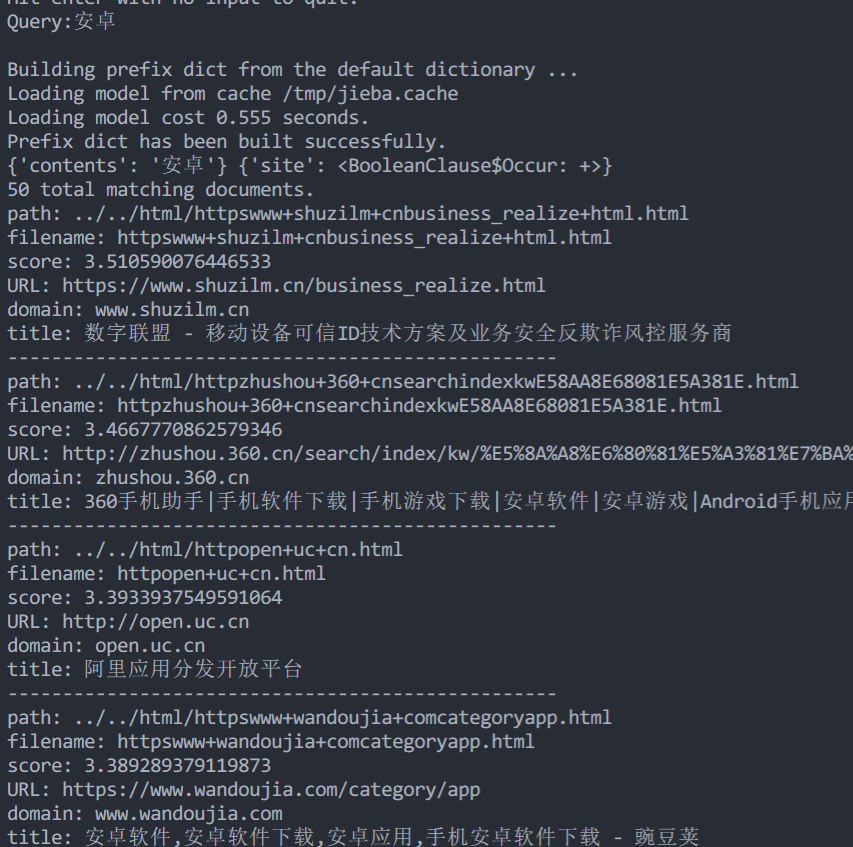
\includegraphics[width=0.6\textwidth]{q00.png}
	\centering
	 \caption{安卓}
\end{figure}
\begin{figure}[H]
	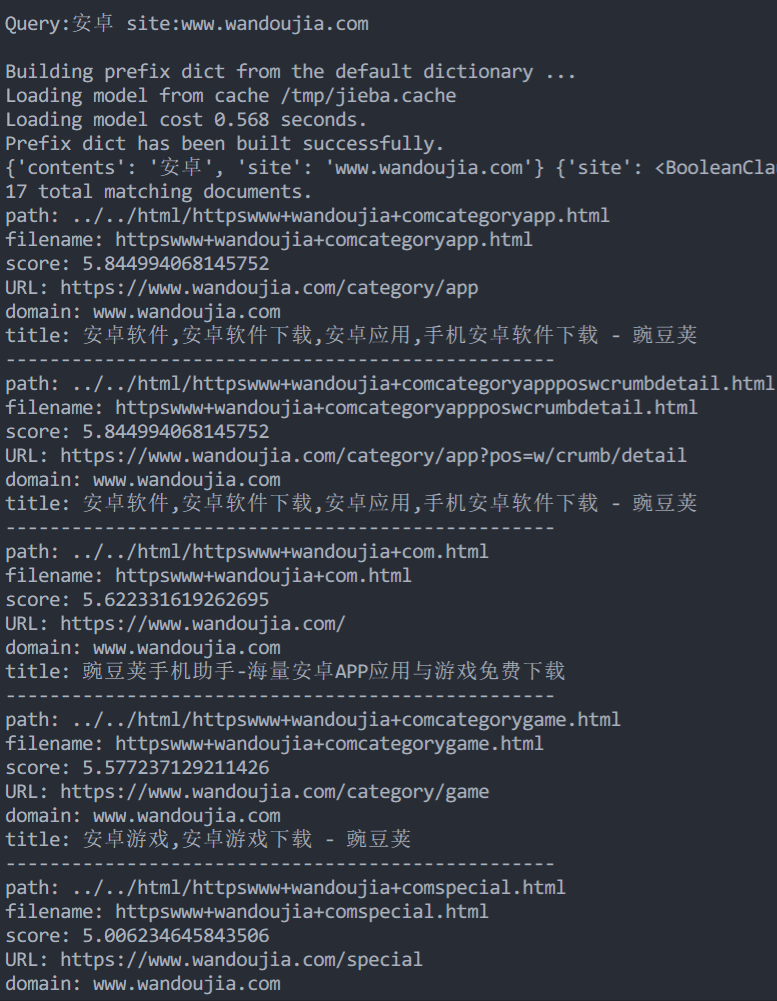
\includegraphics[width=0.6\textwidth]{q01.png}
	\centering
	 \caption{安卓+wandoujia}
\end{figure}

\subsubsection{Example 2}

\begin{figure}[H]
	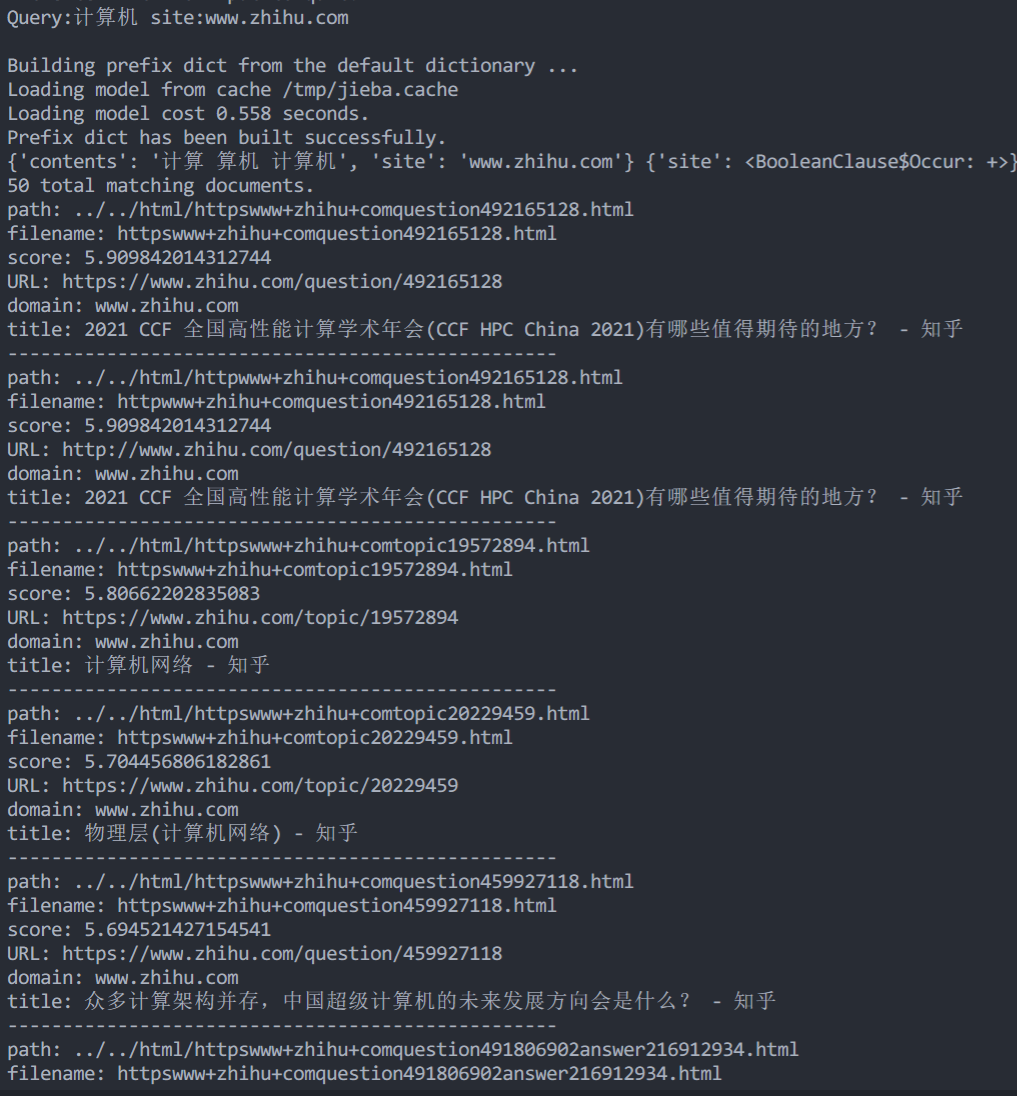
\includegraphics[width=0.6\textwidth]{q10.png}
	\centering
	 \caption{计算机+zhihu}
\end{figure}
\begin{figure}[H]
	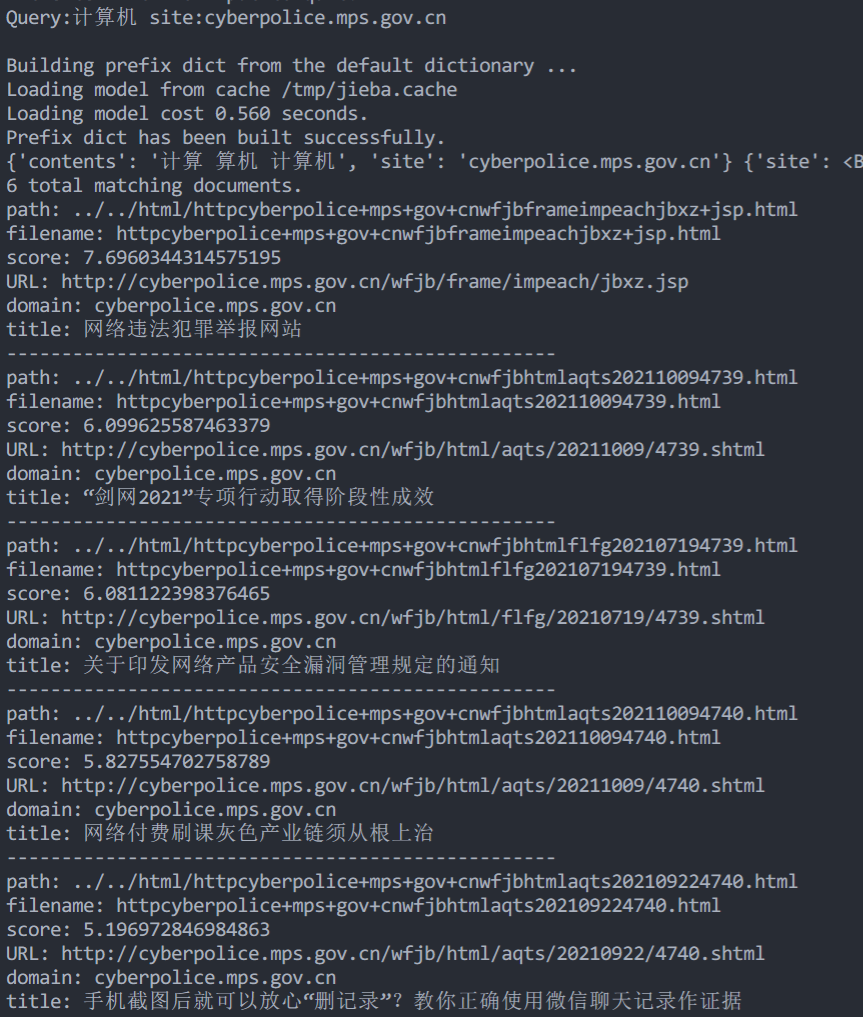
\includegraphics[width=0.6\textwidth]{q11.png}
	\centering
	 \caption{计算机+cyberpolice}
\end{figure}
\subsubsection{Example 3}

\begin{figure}[H]
	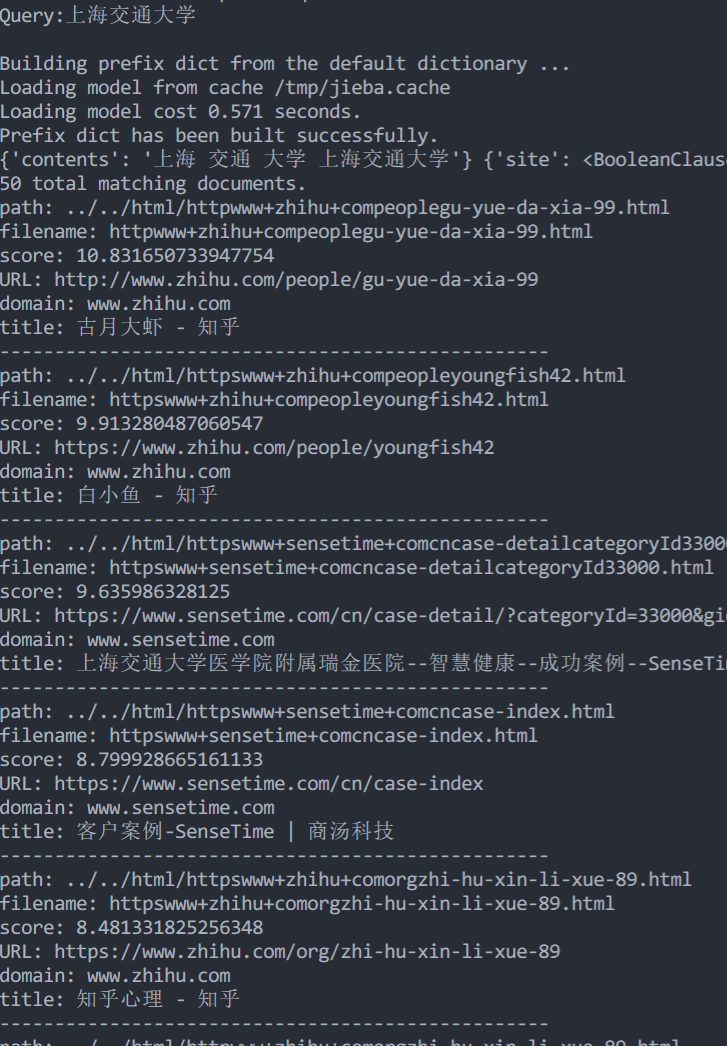
\includegraphics[width=0.6\textwidth]{q20.png}
	\centering
	 \caption{sjtu}
\end{figure}
\begin{figure}[H]
	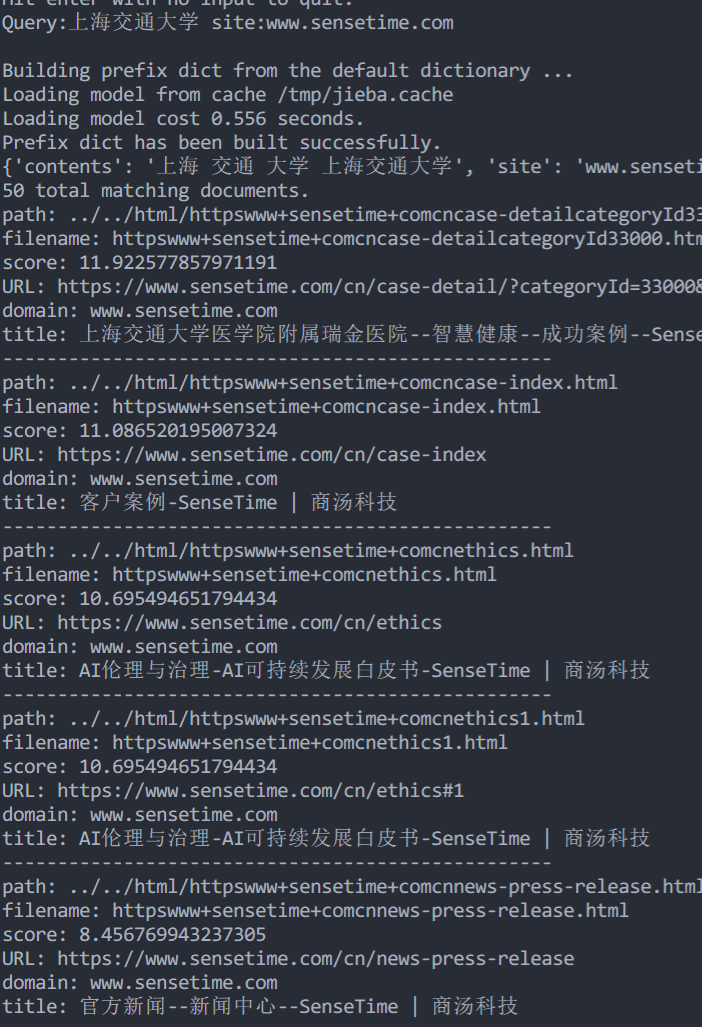
\includegraphics[width=0.6\textwidth]{q21.png}
	\centering
	 \caption{sjtu+sensetime}
\end{figure}
\subsection{图片索引}
\subsubsection{Example 1}
\begin{figure}[H]
	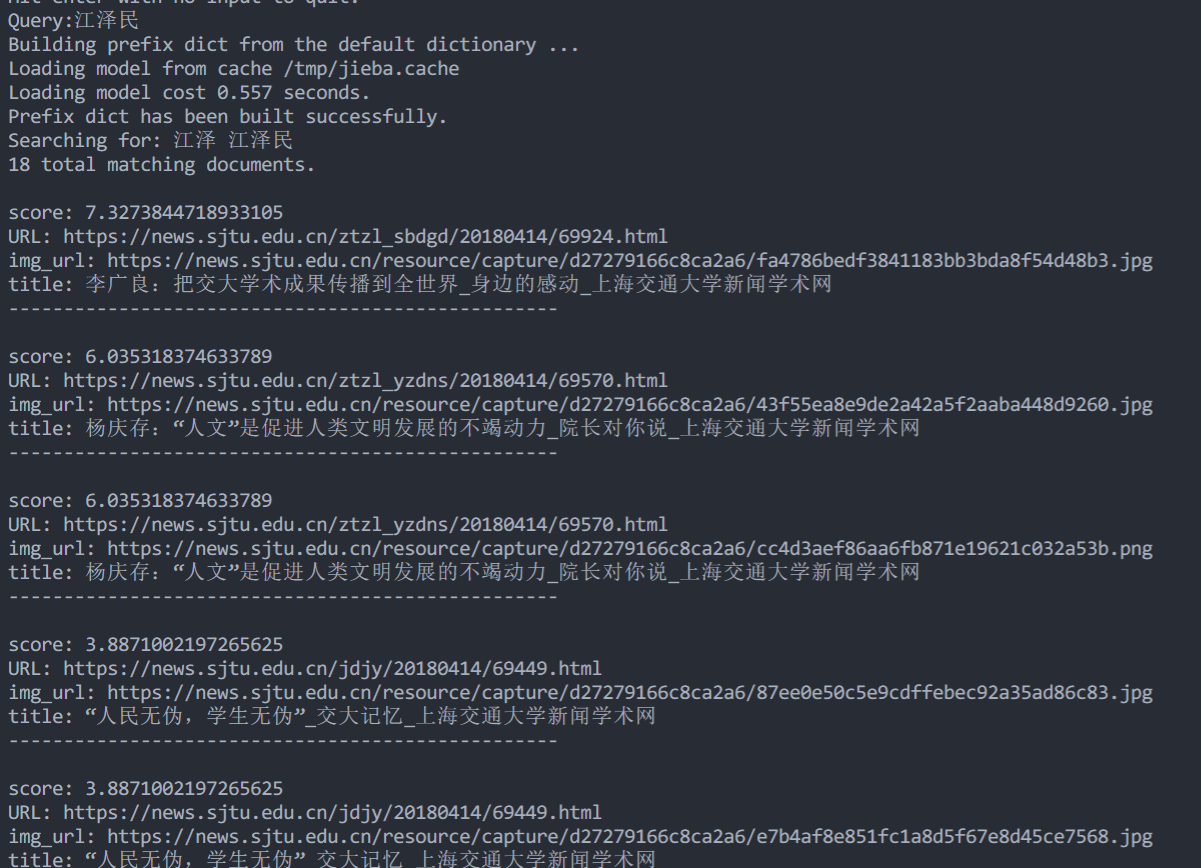
\includegraphics[width=0.7\textwidth]{q30.png}
	\centering
	 \caption{学长}
\end{figure}
\begin{figure}[H]
	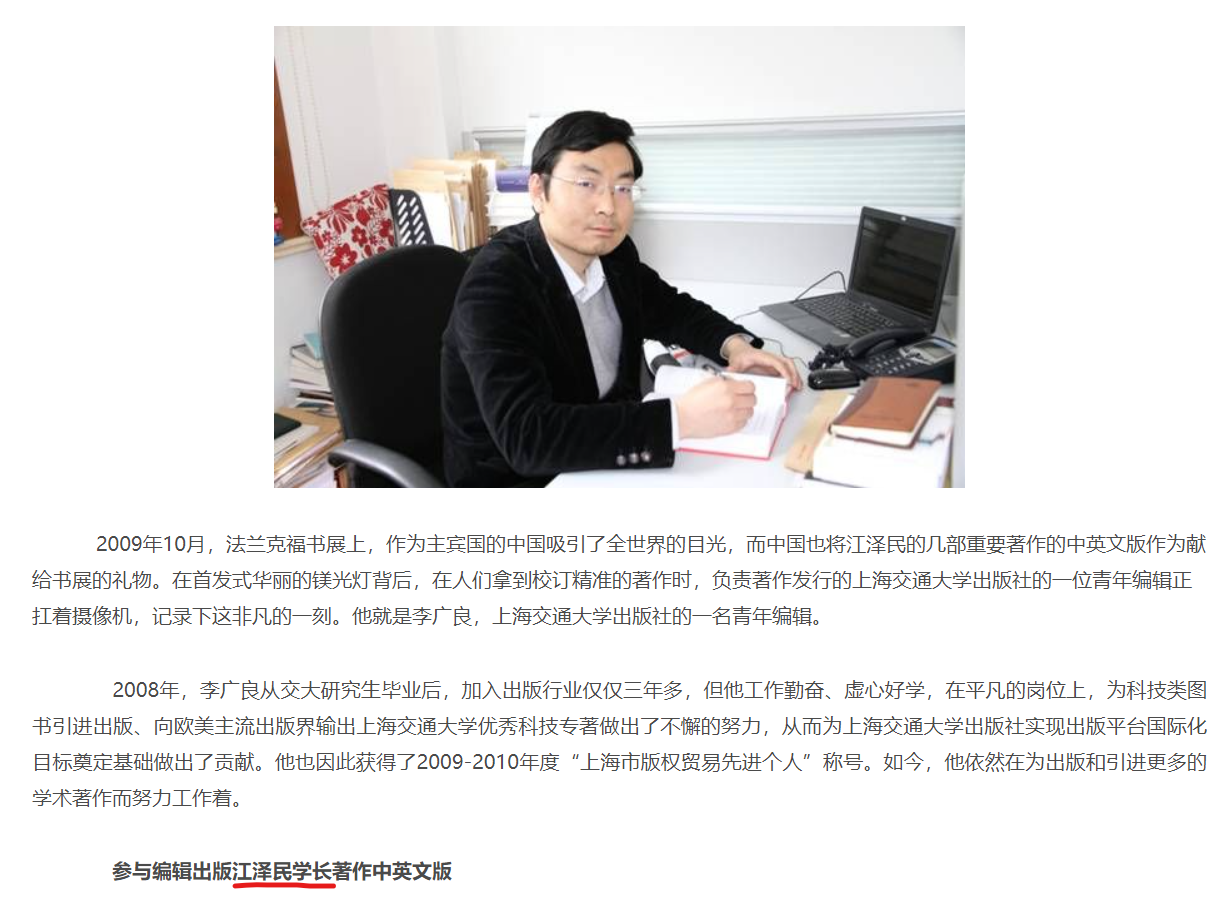
\includegraphics[width=0.7\textwidth]{q31.png}
	\centering
	 \caption{学长}
\end{figure}
\subsubsection{Example 2}
\begin{figure}[H]
	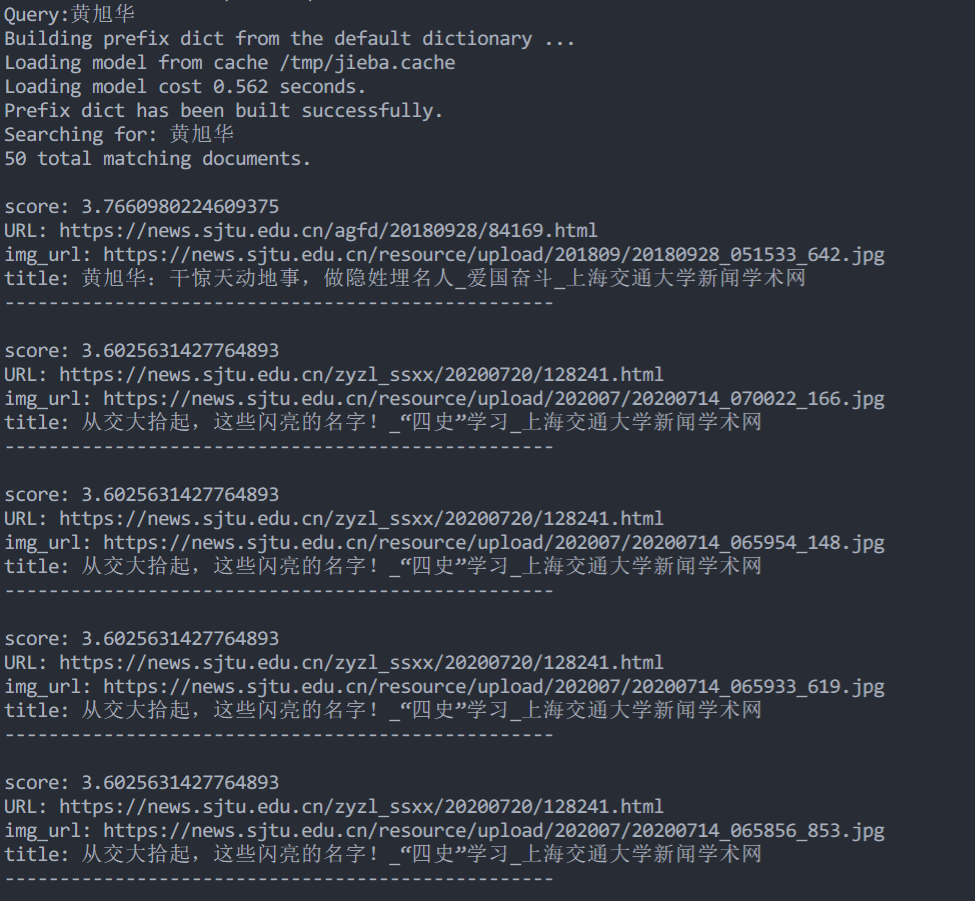
\includegraphics[width=0.6\textwidth]{q40.png}
	\centering
	 \caption{黄旭华}
\end{figure}
\begin{figure}[H]
	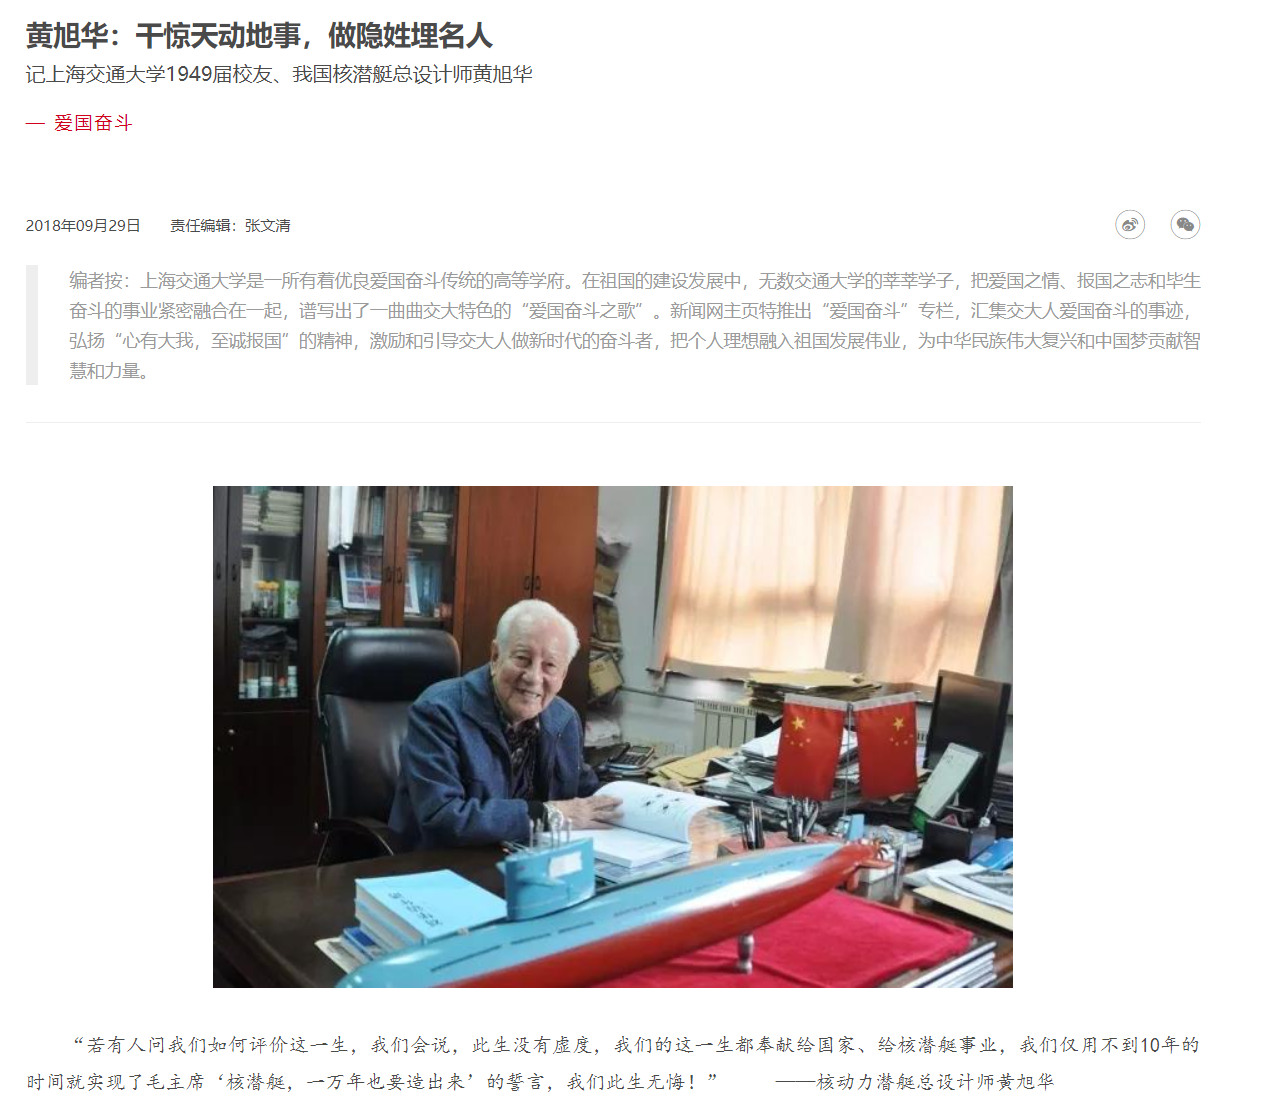
\includegraphics[width=0.6\textwidth]{q41.png}
	\centering
	 \caption{黄旭华}
\end{figure}
\subsubsection{Example 3}
\begin{figure}[H]
	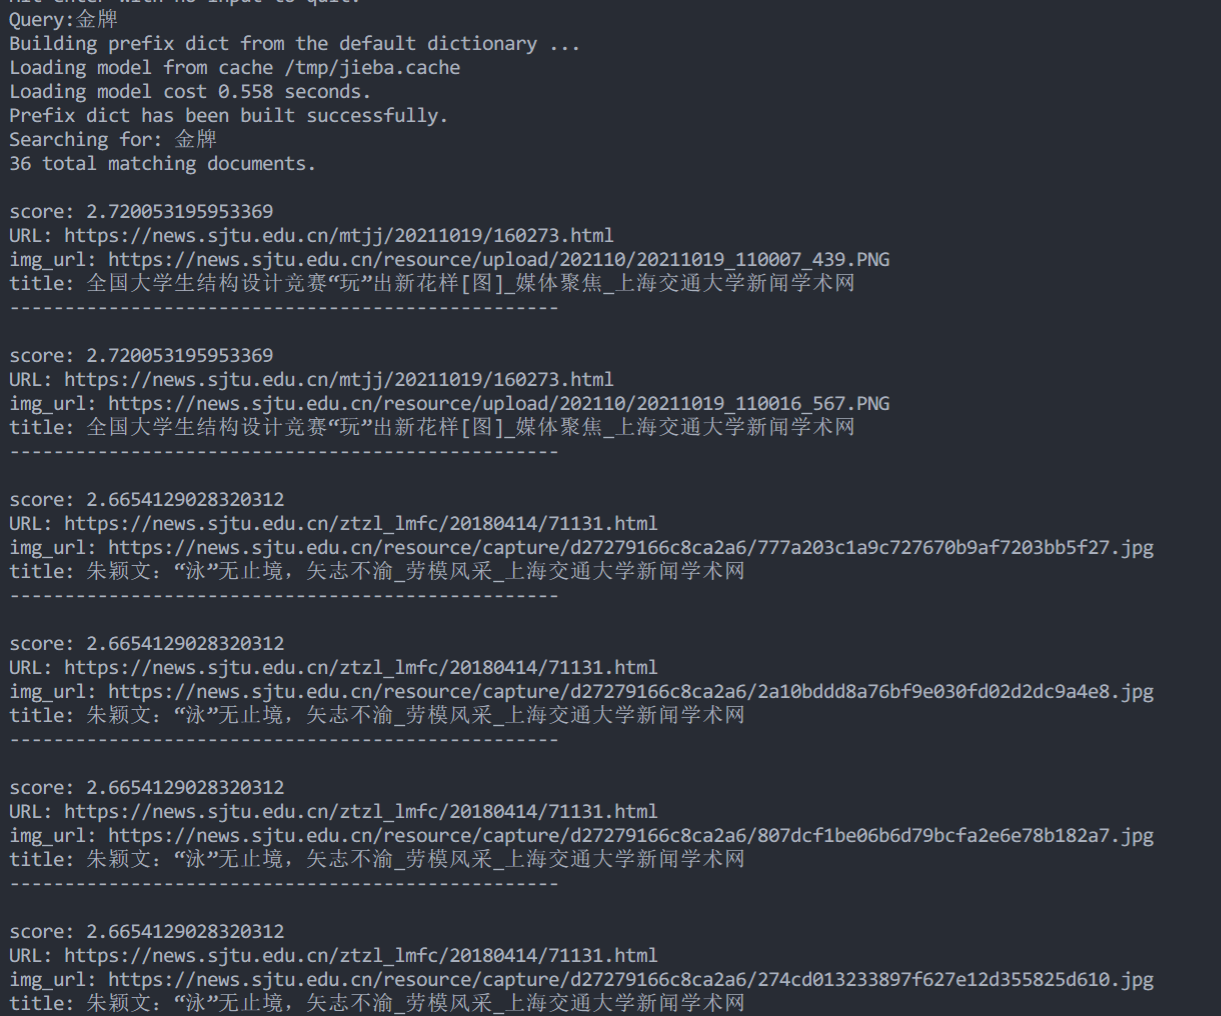
\includegraphics[width=0.7\textwidth]{q50.png}
	\centering
	 \caption{金牌}
\end{figure}
\begin{figure}[H]
	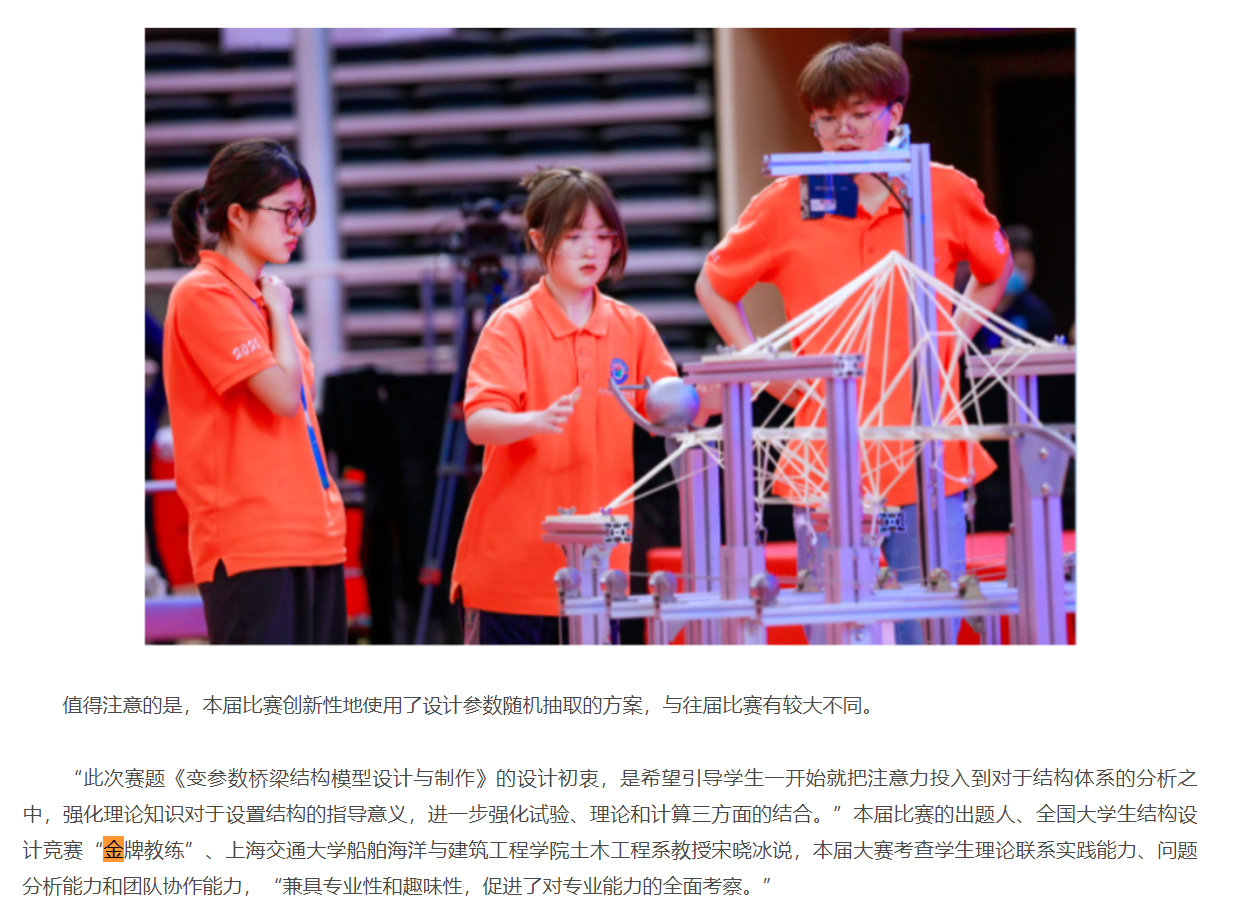
\includegraphics[width=0.7\textwidth]{q51.png}
	\centering
	 \caption{金牌}

\end{figure}

\section{分析与思考}
\begin{itemize}
	\item 在构建索引时,需要特别注意Field的类型,哪些Field是需要index、tokenize的,否则会导致搜索结果出现隐蔽的奇怪错误
	\item 高级搜索可以通过将多个query组合成一个大BooleanQuery实现,其中每个query都可以分别设置搜索内容和布尔要求,甚至可以用不同的analyzer。
	\item 图片索引方面,由于不同网页HTML结构、渲染图片的位置、文字的方位各不相同,实际上要想不借助视觉实现精确定位图片周围的文字十分困难。一些结构简单的网页文字和图片的tag是同层或是隔了几层,但是复杂的网站就不能这么做了,这是用标签siblings的局限性。
\end{itemize}

\end{document}

